\begin{figure}[htb!] 
\centering
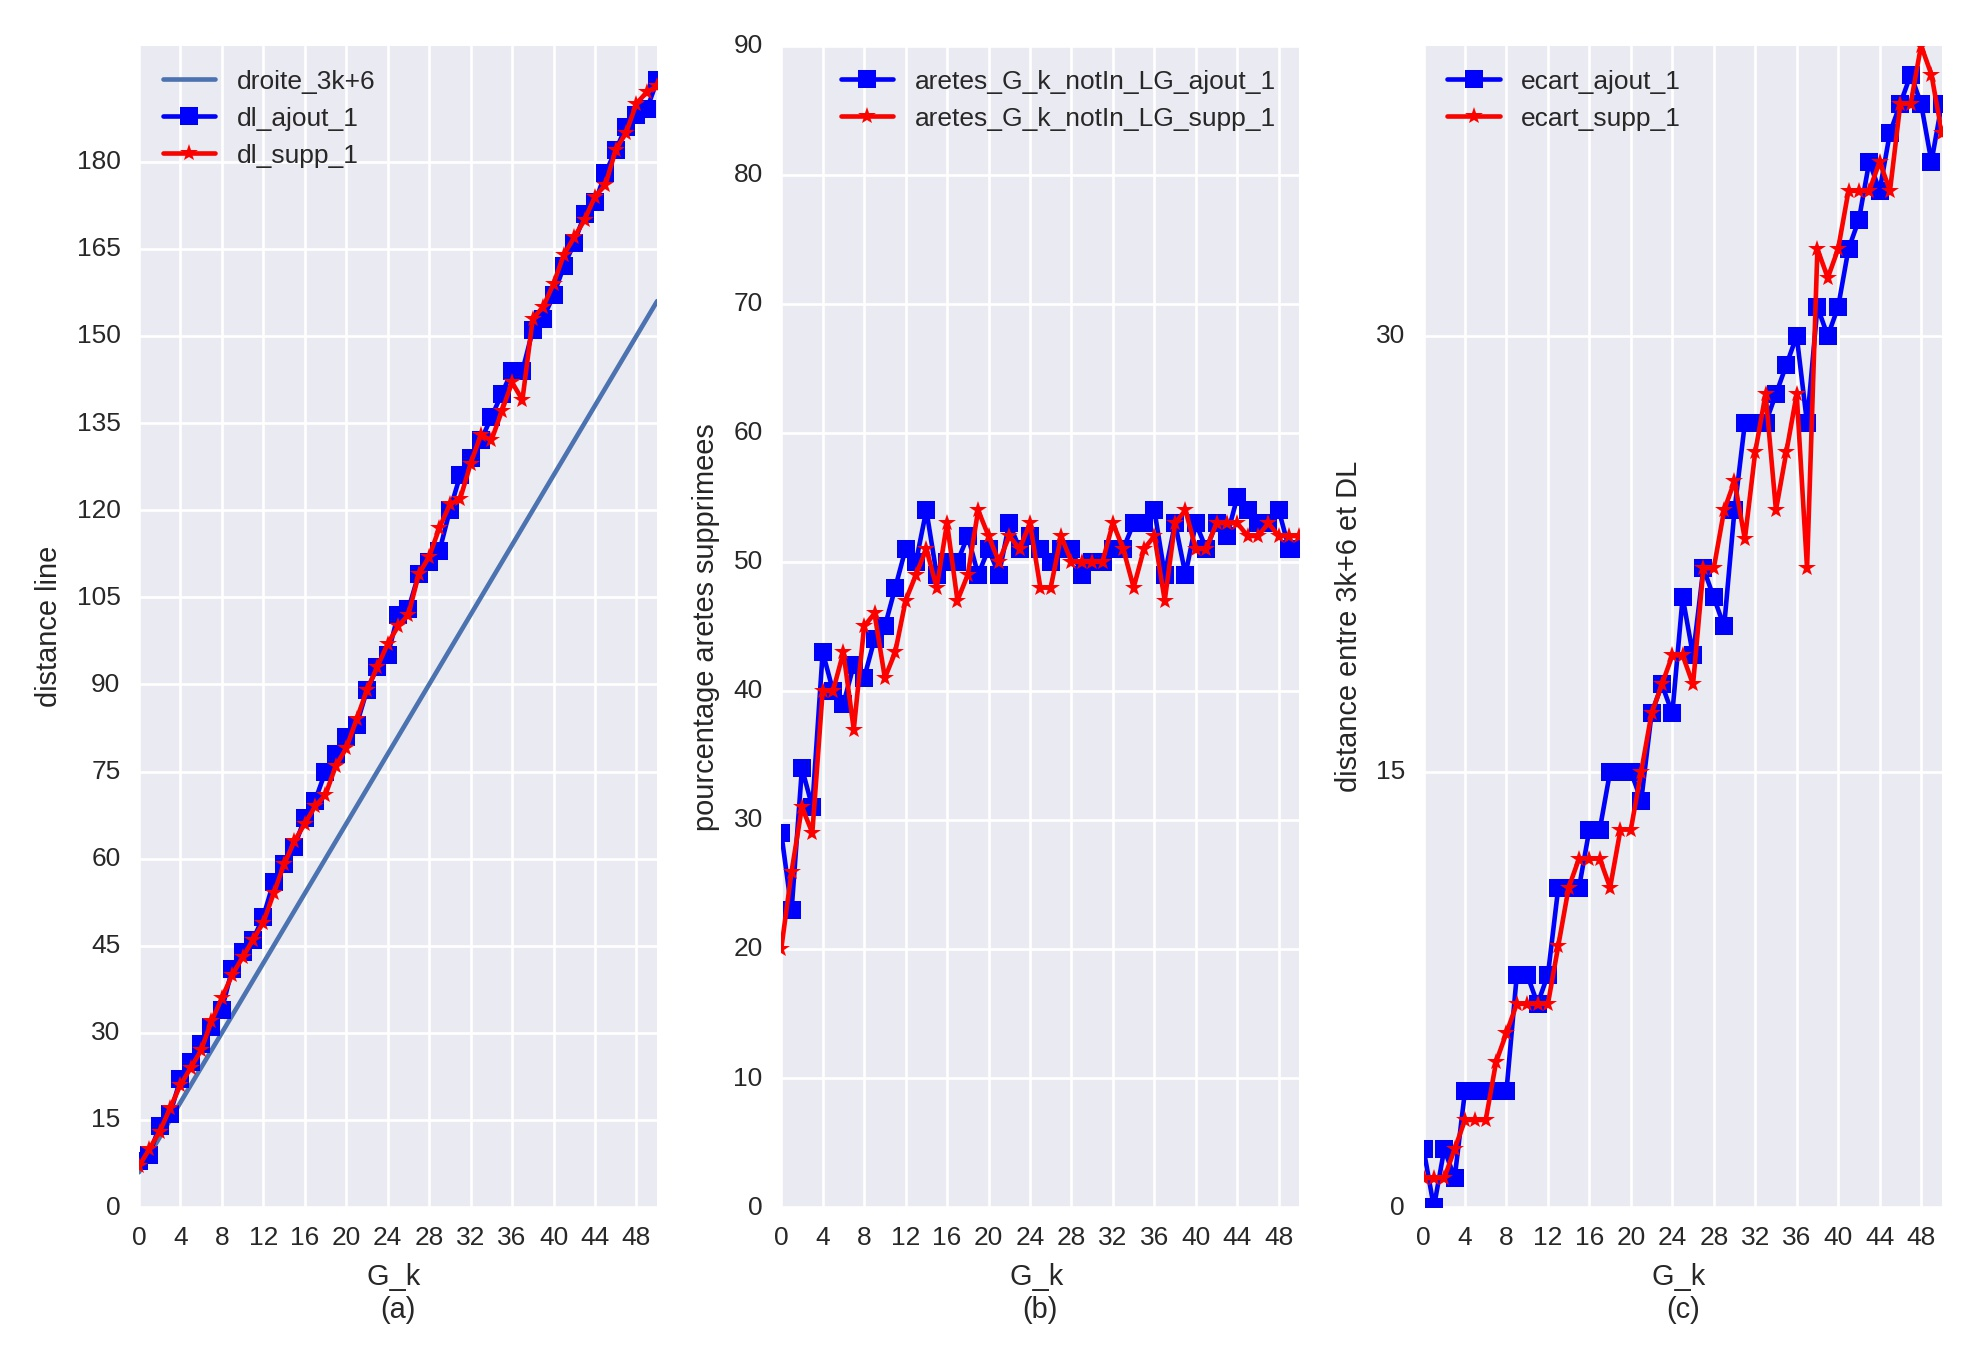
\includegraphics[scale=0.250]{comparaison_prior_ajout_wi_1_supp_wi_1_distance_line_vs_3k_6_graphe_iourte.jpeg}
\caption{  (a) fonction de co\^ut {\em unitaire} : la courbe {\em dl\_ajout\_1} d\'esigne la correction par la priorisation des ar\^etes ajout\'ees avec un poids $\phi^{+} = 1$  pour une ar\^ete ajout\'ee et un poids $\phi^{-} = 1$  pour une ar\^ete supprim\'ee.
 La courbe {\em dl\_supp\_1} d\'esigne la correction par la priorisation des ar\^etes  supprim\'ees avec les co\^uts d'ajout et de suppression d'ar\^etes identiques $\phi^{+} = \phi^{-} = 1$,
 (b) taux de suppression d'ar\^etes dans  $G_0^k$ pour les priorisations  {\em dl\_ajout\_1} et  {\em dl\_supp\_1},
 (c) la diff\'erence de distances line entre les priorisations {\em dl\_ajout\_1} et  {\em dl\_supp\_1}  et la droite $y=3k+6$. }
\label{priorAjout1Supp1} 
\end{figure}

Nous distinguons trois graphiques dans la figure \ref{priorAjout1Supp1}.
Le premier graphique d\'esigne la correction des sommets en supposant que  l'ajout et la suppression d'ar\^etes co\^utent $1$.
%La courbe {\em dl\_ajout\_1} repr\'esente les distances line calcul\'ees en priorisant l'ajout d'ar\^etes pendant la correction. La priorisation consiste \`a attribuer un poids $\phi{+} = 1$ pour des ar\^etes ajout\'ees et un poids $\phi{-} = 1$ pour les ar\^etes supprim\'ees. 
La courbe {\em dl\_ajout\_1} repr\'esente les distances line calcul\'ees en attribuant un poids $\phi^{+} = 1$ pour des ar\^etes ajout\'ees et un poids $\phi^{-} = 1$ pour les ar\^etes supprim\'ees. Le poids $\phi^{+} = 1$ indique que nous priorisons l'ajout d'ar\^etes.
De m\^eme, la courbe {\em dl\_supp\_1} priorise la suppression d'ar\^etes en attribuant  un poids $\phi^{-} = 1$ aux ar\^etes supprim\'ees et un poids $\phi^{+} = 1$ aux ar\^etes ajout\'ees.
La courbe {\em droite\_3k+1} est la droite qui d\'esigne la borne sup\'erieure des distances line.
Le second graphique repr\'esente le nombre d'ar\^etes supprim\'ees dans les graphes $G_k$.
Et le troisi\`eme graphique est celui de l'\'ecart entre la courbe  {\em dl\_ajout\_1}  et la droite $y = 3k+6$  not\'e {\em ecart\_ajout\_1}. Il pr\'esente aussi l'\'ecart {\em  ecart\_supp\_1} entre la courbe  {\em dl\_supp\_1}  et la droite $y = 3k+6$.
\newline
Nous appliquons les m\^emes poids aux op\'erations d'ajout et de suppression d'ar\^etes. Dans les courbes {\em dl\_ajout\_1} et {\em dl\_supp\_1}, l'algorithme de correction ajoute autant d'ar\^etes qu'il n'en supprime. Il ne priorise pas l'ajout d'ar\^etes dans la courbe  {\em dl\_ajout\_1}  et la suppression  d'ar\^etes dans la courbe  {\em dl\_supp\_1}. Ce qui explique la superposition de ces courbes dans le graphique \ref{priorAjout1Supp1}(a). 
De m\^eme, les courbes d'\'ecarts {\em ecart\_ajout\_1} et {\em  ecart\_supp\_1} sont aussi superpos\'ees (voir la figure  \ref{priorAjout1Supp1} (c)) et le taux d'ar\^etes supprim\'ees est relativement identique dans la figure \ref{priorAjout1Supp1} (b).
La suppression massive engendre de nombreux ajouts d'ar\^etes dans les courbes {\em dl\_ajout\_1} et {\em dl\_supp\_1} pour obtenir un line-graphe connexe.

